\documentclass[10pt]{exam}
\usepackage[phy]{template-for-exam}
\usepackage{enumitem,multirow,tikz,multicol}

\title{Car Lab \#1}
\author{Rohrbach}
\date{\today}

\begin{document}
\maketitle

\vspace{-1em}
\section*{Procedure:}
  \begin{enumerate}[label=\alph*),topsep=0pt,itemsep=-1ex,partopsep=1ex,parsep=1ex]
    \item 
      Find a spot on the hallway for your group and mark one-meter intervals on the floor with the dry-erase marker from zero to five meters.
    \item 
      Set the car at the zero mark (the starting line)
    \item
      Run the car.  Make a mark on the ground where the car is at 2, 4, 6, 8, 10, and 12 seconds.
    \item
      Measure how far each mark is from the starting point with your meter stick.  \emph{Make your measurements in meters.}
    \item
      Repeat all of these steps two more times so that you have a total of three trials
    \item 
      Repeat all of these steps for the other car
    \item 
      When you are finished, make sure to use a rag to erase all of the marks on the floor.
  \end{enumerate}

  \paragraph{Pre-Lab:} After reading the procedure, identify each of the following:

    \begin{center}
      \begin{tabular}
        { m{.25\textwidth} | m{.3\textwidth}| m{.25\textwidth} } 
        Independent Variables & 
        Dependent Variables   & 
        Control Variables  \\[6em]
      \end{tabular}
    \end{center}

\vspace{-2em}
\section*{Data}

  \def\cw{.15\textwidth}
  \newcommand{\datatable}{
    \renewcommand{\arraystretch}{1.65}
    \begin{center}
      \begin{tabular}
        {
          |*{4}{>{\centering\arraybackslash}m{\cw}|}
          |>{\centering\arraybackslash}m{\cw}|
        }
        \hline
        \multirow{2}{\cw}
          {\centering Time (s)} & 
        \multicolumn{4}{c|}{Displacement (m)} \\
        \cline{2-5}
        & Trial \#1 & Trial \#2 & Trial \#3 & Average \\
        \hline
        2 &&&&\\
        \hline
        4 &&&&\\
        \hline
        6 &&&&\\
        \hline
        8 &&&&\\
        \hline
        10 &&&&\\
        \hline
        12 &&&&\\
        \hline
      \end{tabular}
    \end{center}
  }

  \noindent
  Red Car:
  \datatable

  \noindent
  Blue Car:
  \datatable

  \paragraph{Graph:} 
    Go to \texttt{www.desmos.com/calculator} to graph your data.  Make sure to submit a link to your graph on Schoology

\begin{multicols}{2}

  \begin{enumerate}[label=\alph*),topsep=0pt,itemsep=-1ex,partopsep=1ex,parsep=1ex]
    \item \label{table} Start by making a table by clicking the “+” icon at the top left.  You will need to create two separate tables.
    \item \label{wrench} Make sure to label the axes using the wrench icon at the right.
    \item \label{zoom} Zoom out so that you can see the whole graph and so that it fills the page.  You can do this using the ``Zoom Fit'' option, but be careful that your fit does not cut off one of the graphs
    \item \label{linear} Create best fit lines for each graph using the ``Linear Regression'' tool
    \item Copy a link to your graph using the export button and clicking ``Share a Snapshot''.  Paste this link on the appropriate place in Schoology.
  \end{enumerate}

  \begin{tikzpicture}
    \node[anchor=north west] at (0,0) 
      {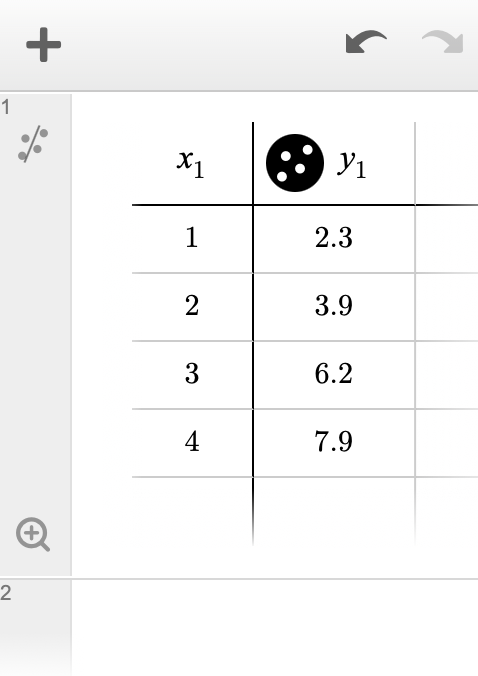
\includegraphics[width=3cm]{desmos1}};


    \node[anchor=north west] at (3.5,0) 
      {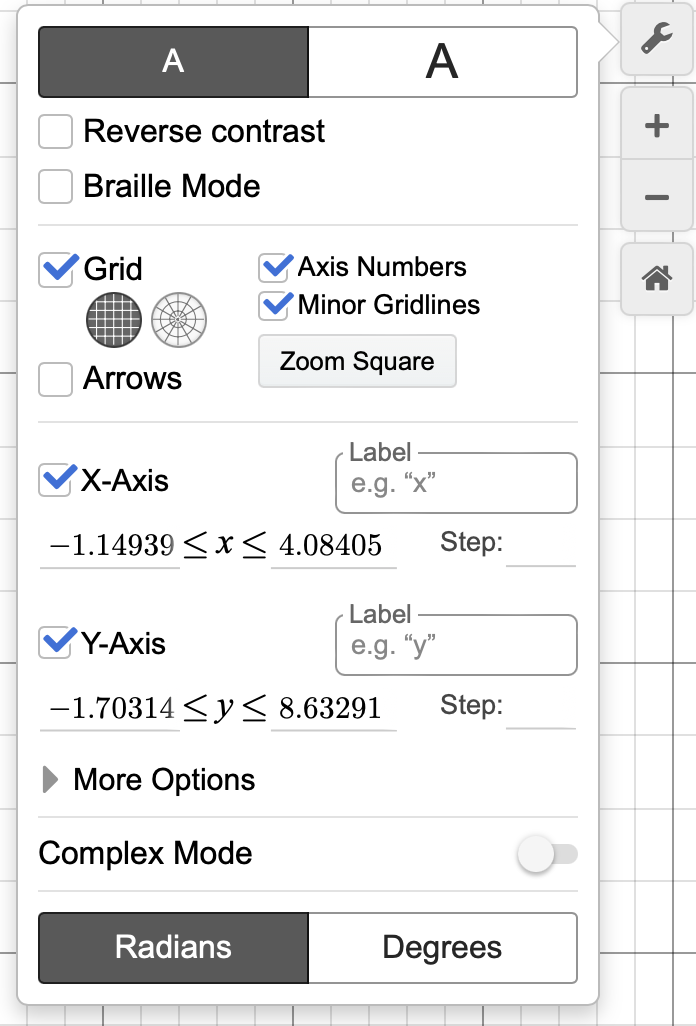
\includegraphics[width=3.5cm]{desmos2}};

        \draw (2,0) 
      node[fill=red!20,rounded corners] (table)
      {\ref{table} Create a table};
    \draw[red] (0.4,-.4) coordinate (a) circle (0.3);
    \draw[<-,red,very thick] (a) +(0.3,0) -- (table.south);

    \node[fill=blue!20,rounded corners] at (2.5,-1.5) (linear) {\ref{linear} Linear Regression};
    \draw[blue] (0.3,-1) coordinate (a) circle (0.3);
    \draw[<-,blue,very thick] (a) +(0.3,0) -- (linear.north);

    \node[fill=green!20,rounded corners] at (2,-2.5) (zoom) {\ref{zoom} Zoom Fit};
    \draw[green, ultra thick] (0.3,-3.5) coordinate (a) circle (0.3);
    \draw[<-,green,very thick] (a) +(0.3,0) -- (zoom.west);

    \node[fill=orange!20,rounded corners] at (4.5,-0.5) (wrench) {\ref{wrench} Axis Labels};
    \draw[orange, ultra thick] (6.9,-.3) coordinate (a) circle (0.3);
    \draw[<-,orange,very thick] (a) +(-0.3,0) -- (wrench.east);

    \draw[->,orange,very thick] (wrench.south) -- (5.2,-2.3);

    \draw[orange, ultra thick, rounded corners] (3.8,-2.3) rectangle ++(2.8,-0.5);
    \draw[orange, ultra thick, rounded corners] (3.8,-3.1) rectangle ++(2.8,-0.5);
  \end{tikzpicture}

\end{multicols}

  \paragraph{Best fit lines:}
    Write down the equations for each of the best fit lines below:

    \vspace{1em}

    Line \#1:

    \vspace{2em}

    Line \#2:
  
    \vspace{1em}

\section*{Analysis}

\begin{questions}

  \question
    What is the physical meaning of the slope of each of the lines?  Explain.
    \vs

  \question
    Just by looking at the graph, how can you tell which car is faster?
    \vs
    
  \question
    How does this graph show that these cars have a constant velocity?
    \vs
  
  \question
    Are your results accurate?  Explain.
    \vs
  
  \question
    Are your results precise?  Explain.
    \vs

  \question
    What were some aspects that limited the accuracy of our graphs and/or our precision?  What could be done to mitigate these in future experiments?
    \vs
  
  


\end{questions}

\end{document}